\chapter{Âm thanh, dao động tử lượng tử và nguyên lý thứ hai}

\lectureoverview{Đích đến là nguyên lý thứ hai, nhưng hai phép tính cụ thể mở đường tới đó. Tốc độ âm thanh kiểm nghiệm cách các đạo hàm nhiệt động học trở thành chuyển động có thể quan sát được. Sau đó, dao động tử điều hòa phơi bày sự thất bại của phân bố đều năng lượng cổ điển đối với các bậc tự do cứng, đồng thời cho thấy cơ học lượng tử kích hoạt các mốt từng cái một như thế nào. Cuối cùng, ta quay lại xung đột có vẻ tồn tại giữa động lực học vi mô thuận nghịch và entropy tăng, dùng dòng chảy trong không gian pha, làm thô, hỗn loạn và sự tái diễn để phát biểu nguyên lý thứ hai như một quy luật có xác suất áp đảo chứ không phải một điều cấm cơ học tuyệt đối không ngoại lệ.}

\section{Lời hứa về nguyên lý thứ hai}

Vấn đề trung tâm thì dễ nêu ra nhưng khó giải thích. Các phương trình Newton là thuận nghịch theo thời gian: nếu một lịch sử vi mô được phép, thì lịch sử đảo ngược thời gian của nó cũng được phép. Tuy vậy, nguyên lý thứ hai lại nói rằng các quá trình vĩ mô có một chiều ưu tiên, được đặc trưng bởi entropy thường tăng. Ta sẽ quay lại sự căng thẳng ấy, nhưng chưa phải ngay bây giờ. Tốt hơn là trước hết hãy thấy cơ học thống kê tạo ra thông tin cụ thể, rồi sau đó gặp, ngay trong một phép tính sơ cấp, câu đố lịch sử đã buộc vật lý cổ điển phải nhường chỗ cho vật lý lượng tử.

Ví dụ thứ nhất là số học và cố ý thô: ước lượng tốc độ âm thanh trong một chất khí loãng. Ví dụ thứ hai là chính xác trong phạm vi các giả thiết của nó: tính năng lượng trung bình của một dao động tử điều hòa trong một bể nhiệt. Dao động tử này sẽ dẫn ta từ phân bố đều năng lượng đến các mức năng lượng lượng tử hóa, từ một mốt đến vô số mốt, và cuối cùng quay lại câu hỏi rằng một hệ nhiều hạt quên trạng thái ban đầu của nó nghĩa là gì.

\section{Thang phân tử của tốc độ âm thanh}

Hãy hình dung một vùng có mật độ hơi cao trong một chất khí loãng. Nó lan ra vì các phân tử rời khỏi vùng đông đúc ấy, nên tốc độ lan truyền của nó phải cùng cỡ với tốc độ phân tử. Theo phân bố đều năng lượng, động năng của một phân tử là \begin{equation}
 \frac{3}{2}k_B T
 =\frac{1}{2}m\expect{v^2},
 \qquad
 \expect{v^2}=\frac{3k_B T}{m}.
 \label{eq:sm7-molecular-speed}
\end{equation} Ở đây, nhiệt độ được đo từ độ không tuyệt đối và \(k_B\) đã được đưa lại vì ta muốn dùng đơn vị phòng thí nghiệm. Lập luận này chỉ là một ước lượng về bậc độ lớn: tốc độ căn trung bình bình phương của phân tử tự nó không phải là tốc độ của một sóng âm tập thể.

Một phép suy luận có hệ thống hơn xét một phần tử khí nhỏ. Các áp suất không bằng nhau trên hai mặt đối diện tác dụng một lực tổng cộng, và gia tốc của nó tỉ lệ nghịch với khối lượng riêng. Kết quả có dạng \begin{equation}
 c_s^2=
 \left(\frac{\partial P}{\partial \rho_m}\right)_{\cal C},
 \qquad
 \rho_m=m\rho,
 \label{eq:sm7-sound-general}
\end{equation} trong đó \(\rho\) là mật độ số và chỉ số dưới \({\cal C}\) xác định điều kiện nhiệt động học mà nhiễu động tuân theo. Phép tính trên bảng dùng \begin{equation}
 P=\rho k_B T
 \quad\Longrightarrow\quad
 \frac{1}{m}
 \left(\frac{\partial P}{\partial\rho}\right)_T
 =\frac{k_B T}{m}.
 \label{eq:sm7-sound-isothermal}
\end{equation} Đây là ước lượng đẳng nhiệt của tốc độ âm thanh. Nó khác \eqref{eq:sm7-molecular-speed} bởi một hệ số \(3\) trong bình phương tốc độ, hay \(\sqrt{3}\) trong chính tốc độ đó.

\begin{figure}[t] \centering
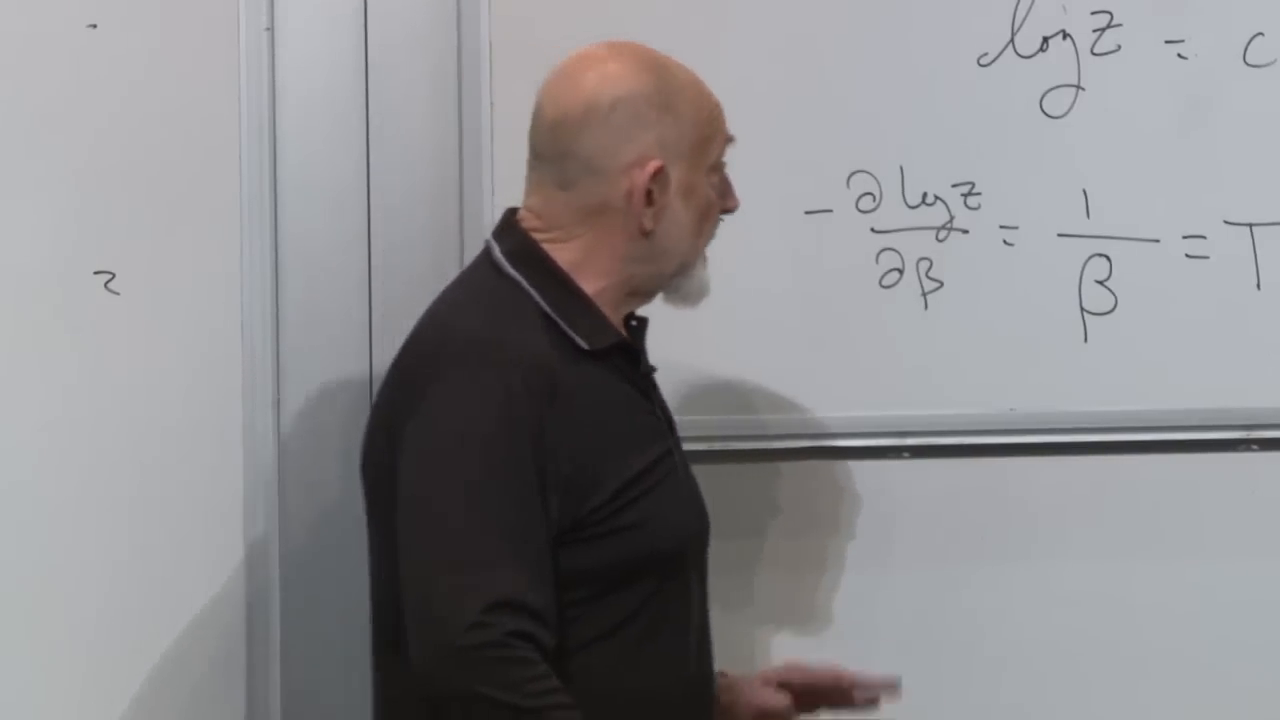
\includegraphics[width=0.90\textwidth]{lecture_07_figure_02.png} \caption{Ước lượng theo tốc độ phân tử, đạo hàm áp suất và phép thế khí lý tưởng được trình bày cùng nhau.} \lectureframe{00:08:55} \end{figure}

Có một sự tinh chỉnh quan trọng. Một sóng âm biên độ nhỏ thông thường nén và làm loãng chất khí nhanh hơn việc nhiệt có thể truyền giữa các phần tử lân cận. Vì vậy, chuyển động cục bộ xấp xỉ đoạn nhiệt chứ không phải đẳng nhiệt: \begin{equation}
 c_s^2=
 \left(\frac{\partial P}{\partial\rho_m}\right)_S.
 \label{eq:sm7-sound-adiabatic}
\end{equation} Đối với một khí lý tưởng có chỉ số đoạn nhiệt \(\gamma\), \begin{equation}
 P\rho_m^{-\gamma}=\text{constant},
 \qquad
 c_s^2=\gamma\frac{P}{\rho_m}
       =\gamma\frac{k_B T}{m}.
 \label{eq:sm7-sound-ideal-adiabatic}
\end{equation} Đối với không khí lưỡng nguyên tử ở nhiệt độ phòng, \(\gamma\simeq 7/5\). Vì thế, phép tính ở nhiệt độ cố định là một ước lượng đầu tiên hữu ích, còn đạo hàm đoạn nhiệt cung cấp sự tinh chỉnh phù hợp về mặt vật lý.

Dùng các giá trị thô \begin{equation}
\begin{aligned}
 k_B&\simeq1.3\times10^{-23}\ {\rm J\,K^{-1}},
 &T&\simeq300\ {\rm K},\\
 m_{\rm air}&\simeq4\times10^{-26}\ {\rm kg}.&&
\end{aligned}
 \label{eq:sm7-air-data}
\end{equation}, ước lượng theo phân tử vào khoảng \(500\ {\rm m\,s^{-1}}\). Ở đây nhiệt độ phải là nhiệt độ tuyệt đối tính bằng kelvin, không phải một thang đo lệch gốc như Fahrenheit. Tốc độ âm thanh quen thuộc có cỡ \(300\ {\rm m\,s^{-1}}\), và công thức khí lý tưởng đoạn nhiệt cho khoảng \(340\ {\rm m\,s^{-1}}\) ở nhiệt độ phòng. Vì vậy, phép tính thô đã tìm ra đúng bậc độ lớn vật lý.

\begin{figure}[t] \centering
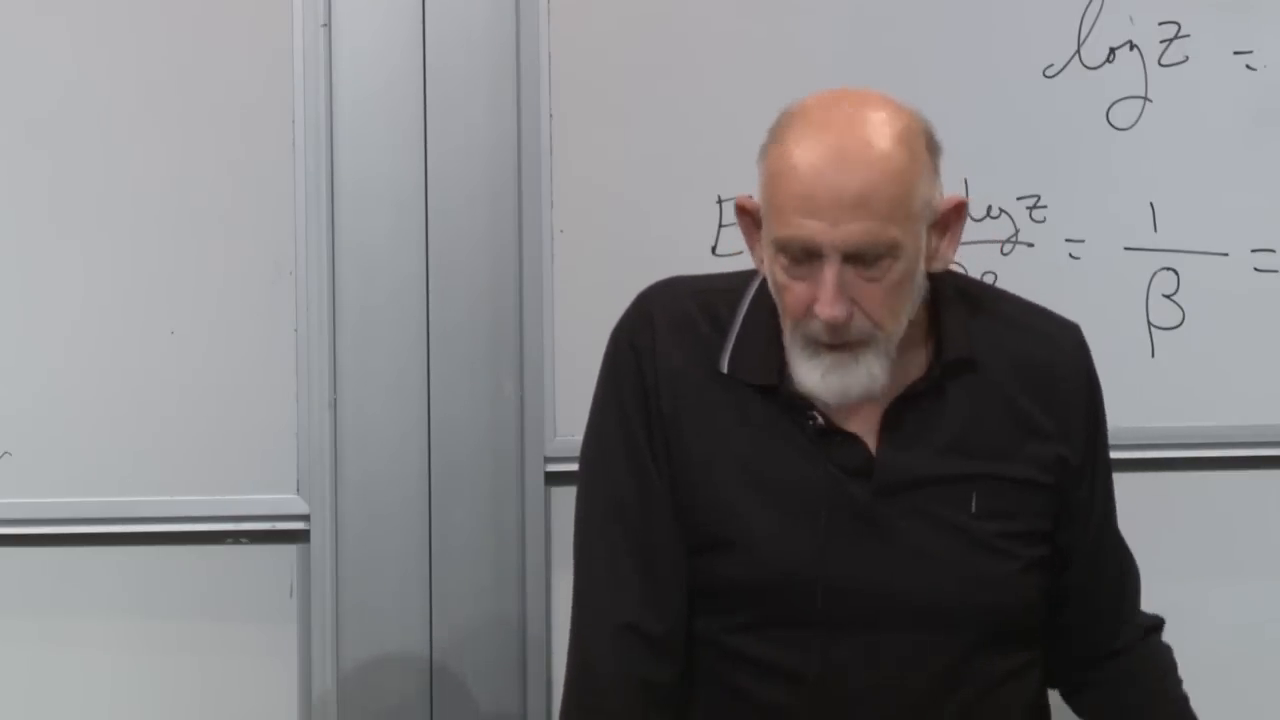
\includegraphics[width=0.90\textwidth]{lecture_07_figure_03.png} \caption{Ước lượng cho không khí ở nhiệt độ phòng dùng hằng số Boltzmann, một khối lượng phân tử hiệu dụng gần \(30\) khối lượng proton, và \(T\simeq300\ {\rm K}\).} \lectureframe{00:10:55} \end{figure}

Từ rất lâu trước khi có được một mô tả vi mô, người ta đã có thể xác định tốc độ âm thanh từ các phép đo áp suất theo khối lượng riêng. Lập luận thống kê bổ sung một cách diễn giải rất đáng chú ý rằng tốc độ vĩ mô ấy được ấn định bởi tốc độ nhiệt của từng phân tử riêng lẻ.

\begin{classroomqa} \audiencequestion{Có cần cộng neutron vào khối lượng phân tử không, và con số \(14\) đối với nitơ có chỉ tính proton thôi không?} \lecturerresponse{Nguyên tử lượng được nêu ra đã tính cả proton lẫn neutron. Phân tử nitơ gồm hai nguyên tử có nguyên tử lượng xấp xỉ \(14\), nên khối lượng của nó xấp xỉ \(28\) khối lượng proton; làm tròn \(28\) thành \(30\) là đủ cho ước lượng này. \lecturetimestamp{00:10:58--00:11:16}} \end{classroomqa}

\begin{classroomqa} \audiencequestion{Hệ số \(3\) xuất phát từ ba phương tịnh tiến, trong khi âm thanh truyền theo một phương. Có phải vì vậy phải bỏ hệ số \(3\) đi không?} \lecturerresponse{Điều đó đúng là nhắc ta không được đồng nhất tốc độ căn trung bình bình phương ba chiều của phân tử với một tốc độ lan truyền một chiều. Lập luận mở đầu chỉ là một bức tranh bậc độ lớn. Câu trả lời chặt chẽ xuất phát từ đạo hàm áp suất, cùng với điều kiện nhiệt động học thích hợp cho sóng. \lecturetimestamp{00:11:12--00:12:00}} \end{classroomqa}

\begin{classroomqa} \audiencequestion{Đạo hàm đó có giả sử rằng nhiệt độ vẫn không đổi trong khi sóng truyền không?} \lecturerresponse{Phép thế khí lý tưởng được trình bày đúng là đã giả sử như vậy. Giữ nhiệt độ cố định là một ước lượng tạm thời hợp lý cho một nhiễu động rất nhỏ; sự tinh chỉnh chuẩn là âm thanh thông thường xấp xỉ đoạn nhiệt, thay đạo hàm đẳng nhiệt bằng \(\left(\partial P/\partial\rho_m\right)_S\). \lecturetimestamp{00:12:59--00:14:01}} \end{classroomqa}

\begin{classroomqa} \audiencequestion{Nếu biến thiên áp suất và khối lượng riêng đều nhỏ, điều đó có làm đạo hàm của chúng nhỏ đi không?} \lecturerresponse{Không. Đạo hàm là tỉ số của hai biến thiên nhỏ trong giới hạn vi phân. Cả \(\delta P\) lẫn \(\delta\rho\) đều có thể nhỏ trong khi \(\delta P/\delta\rho\) vẫn hữu hạn và quyết định tốc độ của sóng. \lecturetimestamp{00:14:03--00:14:23}} \end{classroomqa}

\begin{classroomqa} \audiencequestion{Tốc độ âm thanh có nên tăng khi chất khí bị nén lại, như khi ta đi từ khí về phía lỏng hay rắn không?} \lecturerresponse{Có. Đạo hàm được lấy tại trạng thái đang xét, và \(P(\rho,T)\) không nhất thiết còn tuyến tính. Khi các phân tử bị ép sát nhau, phương trình trạng thái trở nên phi lý tưởng và \(\partial P/\partial\rho\) có thể tăng lên đáng kể. \lecturetimestamp{00:14:25--00:15:13}} \end{classroomqa}

\begin{classroomqa} \audiencequestion{Giá trị \(500\ {\rm m\,s^{-1}}\) có thể dùng ở mọi áp suất không?} \lecturerresponse{Không. Nó thuộc về miền mật độ thấp, nơi phương trình khí lý tưởng là một xấp xỉ hữu ích. Một khi các lũy thừa cao hơn của mật độ đi vào \(P(\rho,T)\), đạo hàm, và do đó tốc độ âm thanh, sẽ phụ thuộc vào áp suất và khối lượng riêng. \lecturetimestamp{00:15:14--00:16:29}} \end{classroomqa}

\begin{classroomqa} \audiencequestion{Bức tranh ban đầu về việc âm thanh lan ra với tốc độ xấp xỉ tốc độ phân tử có cũng thất bại khi mật độ tăng lên không?} \lecturerresponse{Có lẽ có. Bức tranh đó được xây dựng riêng cho chất khí loãng. Ở mật độ cao, các tương tác tập thể trở nên ngày càng quan trọng, và đó chính là lý do đạo hàm của phương trình trạng thái là mô tả tổng quát hơn. \lecturetimestamp{00:16:32--00:16:53}} \end{classroomqa}

\begin{classroomqa} \audiencequestion{Vì sao khối lượng của phân tử nitơ lại được viết là xấp xỉ \(30\) khối lượng proton thay vì \(28\)?} \lecturerresponse{Chỉ cần độ chính xác số phù hợp với phép ước lượng, nên \(28\) đã được làm tròn thành \(30\). Chia ước lượng ban đầu \(500\ {\rm m\,s^{-1}}\) cho \(\sqrt{3}\simeq1.7\) cũng đưa nó lại gần \(300\ {\rm m\,s^{-1}}\), mặc dù đạo hàm đoạn nhiệt mới là cách chặt chẽ để tính hiệu chỉnh đó. \lecturetimestamp{00:16:54--00:17:27}} \end{classroomqa}

\section{Một dao động tử cổ điển trong một bể nhiệt}

Giờ ta thay phân tử chuyển động tịnh tiến tự do bằng một dao động tử điều hòa và coi mọi thứ còn lại là một bể nhiệt. Hình dung trực tiếp là một khối lượng gắn với lò xo, nhưng mô hình này rộng hơn nhiều. Một mốt của khoang điện từ dao động; các nguyên tử trong tinh thể dao động; gần như mọi hệ ổn định bị lệch nhẹ khỏi cân bằng đều thực hiện chuyển động điều hòa ở bậc dẫn đầu.

Với \(x\) được đo từ vị trí cân bằng, xung lượng \(p\), khối lượng \(m\) và hằng số lò xo \(\kappa\), Hamiltonian là \begin{equation}
 H(x,p)=\frac{p^2}{2m}+\frac{\kappa x^2}{2},
 \qquad
 \omega=\sqrt{\frac{\kappa}{m}}.
 \label{eq:sm7-classical-hamiltonian}
\end{equation} Bể nhiệt ấn định \(T\), và từ đây ta lại dùng \(k_B=1\), nên \(\beta=1/T\). Một dao động tử cân bằng nhiệt với phòng có nhiệt độ gần \(300\ {\rm K}\); một dao động tử nhúng trong heli lỏng chỉ có nhiệt độ vài kelvin. Một lò xo giả định đặt ở tâm Mặt Trời sẽ không thể tồn tại như một lò xo, nhưng ví dụ này làm rõ vai trò của môi trường. Trọng số Boltzmann phân tích thành nhân tử: \begin{equation}
 e^{-\beta H}
 =e^{-\beta p^2/(2m)}
  e^{-\beta\kappa x^2/2}.
 \label{eq:sm7-factorized-weight}
\end{equation}

\begin{figure}[t] \centering
\includegraphics[width=0.90\textwidth]{lecture_07_figure_04.png} \caption{Một dao động tử khối lượng-lò xo và Hamiltonian của nó gồm động năng cộng thế năng.} \lectureframe{00:20:55} \end{figure}

Không giống khí tự do, tích phân theo vị trí không chỉ đơn thuần cho ra thể tích của bình chứa. Thế phục hồi gán trọng số cho mỗi li độ:
\begin{equation}
 Z_{\rm cl}
 =\frac{1}{h}\int_{-\infty}^{\infty}dp
             \int_{-\infty}^{\infty}dx\,
 e^{-\beta p^2/(2m)}
 e^{-\beta\kappa x^2/2}.
 \label{eq:sm7-classical-z}
\end{equation}
Thừa số \(1/h\) làm cho hàm phân hoạch cổ điển một chiều trở thành không thứ nguyên. Nó được lược bỏ trong phép tính trên bảng vì không phụ thuộc vào \(\beta\) và không thể ảnh hưởng đến năng lượng trung bình.

\begin{figure}[t]
\centering
\includegraphics[width=0.90\textwidth]{lecture_07_figure_05.png}
\caption{Hàm phân hoạch của dao động tử cổ điển được tách thành các tích phân Gauss theo động lượng và theo li độ.}
\lectureframe{00:22:55}
\end{figure}

Đối với tích phân theo động lượng, đặt
\begin{equation}
 q=\sqrt{\frac{\beta}{2m}}\,p,
 \qquad
 dp=\sqrt{\frac{2m}{\beta}}\,dq.
 \label{eq:sm7-p-gaussian-substitution}
\end{equation}
Đối với tích phân theo vị trí, đặt
\begin{equation}
 y=\sqrt{\frac{\beta\kappa}{2}}\,x,
 \qquad
 dx=\sqrt{\frac{2}{\beta\kappa}}\,dy.
 \label{eq:sm7-x-gaussian-substitution}
\end{equation}
Vì \(\int_{-\infty}^{\infty}e^{-u^2}\,du=\sqrt{\pi}\), tích phân không gian pha không chuẩn hóa được dùng trên bảng là
\begin{equation}
 \int dp\,dx\,e^{-\beta H}
 =\frac{2\pi}{\beta}\sqrt{\frac{m}{\kappa}}
 =\frac{2\pi}{\beta\omega}.
 \label{eq:sm7-classical-z-unnormalized}
\end{equation}
Khi khôi phục ô không gian pha,
\begin{equation}
 Z_{\rm cl}=\frac{2\pi}{h\beta\omega}
           =\frac{1}{\beta\hbar\omega}.
 \label{eq:sm7-classical-z-normalized}
\end{equation}

Đối với năng lượng, chỉ sự phụ thuộc vào \(\beta\) mới quan trọng:
\begin{equation}
 \begin{aligned}
 \log Z_{\rm cl}&=\text{constant}-\log\beta,\\
 \expect{H}
 &=-\frac{\partial\log Z_{\rm cl}}{\partial\beta}\\
 &=\frac{1}{\beta}=T.
 \end{aligned}
 \label{eq:sm7-classical-energy}
\end{equation}

\begin{figure}[t]
\centering
\includegraphics[width=0.90\textwidth]{lecture_07_figure_06.png}
\caption{Chuỗi suy luận cổ điển hoàn chỉnh trên bảng bên phải: phép tách Gauss, \(Z\propto(\beta\omega)^{-1}\), và \(\expect{H}=1/\beta=T\).}
\lectureframe{00:30:15}
\end{figure}

Không có thừa số \(3\) vì đây là một dao động tử trong một chiều không gian. Cũng không còn thừa số \(1/2\) nào nữa, vì có hai hạng bậc hai độc lập. Mỗi tích phân Gauss đóng góp \(T/2\):
\begin{equation}
 \expect{K}=\frac{T}{2},
 \qquad
 \expect{U}=\frac{T}{2},
 \qquad
 \expect{H}=T.
 \label{eq:sm7-equipartition-oscillator}
\end{equation}
Đây là nguyên lý phân bố đều ở dạng hữu ích nhất của nó: mọi hạng bậc hai độc lập trong Hamilton cổ điển đều đóng góp \(T/2\).

Kết quả này không phụ thuộc cả \(m\) lẫn \(\kappa\). Bản thân chuyển động thì có phụ thuộc vào các tham số đó:
\begin{equation}
 \expect{p^2}=mT,
 \qquad
 \expect{x^2}=\frac{T}{\kappa},
 \qquad
 \expect{\dot{x}^2}=\frac{T}{m}.
 \label{eq:sm7-classical-fluctuations}
\end{equation}
Vì vậy, khối lượng lớn hơn chuyển động chậm hơn và lò xo cứng hơn có biên độ nhỏ hơn, mặc dù năng lượng trung bình vẫn là \(T\).
Điều đó trở nên đáng băn khoăn khi \(\kappa\) được làm lớn đến mức phi thường. Một lò xo quá cứng để chuyển động đáng lẽ phải giống như một ràng buộc bị đóng băng, vậy mà phân bố đều cổ điển vẫn gán cho nó năng lượng \(T\).

\begin{classroomqa}
\audiencequestion{Khi \(\kappa\to\infty\), hàm phân hoạch tiến về không. Làm sao vẫn có thể dùng logarit của nó?}
\lecturerresponse{Giữ \(\kappa\) hữu hạn nhưng lớn tùy ý. Đóng góp của nó vào \(\log Z\) là cộng tính và không phụ thuộc vào \(\beta\), nên đạo hàm theo \(\beta\) vẫn cho \(T\). Sự vướng mắc ở giới hạn đó là có thật: phép tính cổ điển là tự nhất quán về nội tại, nhưng nó bỏ sót một đặc điểm của tự nhiên cần thiết cho các dao động tử rất cứng.
\lecturetimestamp{00:34:01--00:34:54}}
\end{classroomqa}

\begin{classroomqa}
\audiencequestion{Hàm phân hoạch của khí lý tưởng cần một \(N!\). Ở đây có nên có một giai thừa tương tự không?}
\lecturerresponse{Không. Ta đang xét một dao động tử được chỉ định cụ thể, chứ không hoán vị \(N\) hạt giống hệt nhau. Đối với nhiều mode độc lập có nhãn, các hàm phân hoạch nhân với nhau. Một thừa số bất khả phân biệt thuộc về một bài toán đếm khác.
\lecturetimestamp{00:35:03--00:35:40}}
\end{classroomqa}

\section{Vì sao nguyên lý phân bố đều cổ điển từng là một cuộc khủng hoảng}

Các phân tử thực không phải là những điểm vô cấu trúc. Một phân tử hai nguyên tử chứa một liên kết có thể dao động, do đó có một dao động tử nội. Một cách đếm cổ điển ngây thơ sẽ gán cho mode đó thêm năng lượng nhiệt ngay cả ở nhiệt độ thông thường. Trong một phép đếm cố ý giản lược, việc kích hoạt một dao động tử dao động nâng năng lượng từ \(3T/2\) lên hướng tới \(5T/2\). Việc hạch toán chính xác nhiệt dung còn phải tính đến các bậc tự do quay và phân biệt năng lượng với đạo hàm của nó theo nhiệt độ. Sự kiện thực nghiệm mang tính quyết định thì đơn giản hơn:
các mode nội cứng đã không đóng góp ở nhiệt độ thấp như phân bố đều cổ điển đòi hỏi.

Ta có thể phủ nhận rằng phân tử có cấu trúc bên trong, điều đó là phi lý, hoặc thừa nhận rằng cơ học cổ điển còn thiếu một thành phần. Thành phần đó là cơ học lượng tử. Ta cần rất ít từ nó: chỉ cần việc một dao động tử điều hòa có các mức năng lượng cách đều.

\section{Dao động tử lượng tử}

Trước hết hãy dịch gốc năng lượng và viết phổ kích thích dưới dạng
\begin{equation}
 E_n^{\rm exc}=n\hbar\omega,
 \qquad n=0,1,2,\ldots.
 \label{eq:sm7-shifted-spectrum}
\end{equation}
Hàm phân hoạch bây giờ là một tổng đúng nghĩa chứ không phải một tích phân trên không gian pha:
\begin{align}
 Z_{\rm exc}
 &=\sum_{n=0}^{\infty}e^{-\beta n\hbar\omega} \notag\\
 &=1+x+x^2+\cdots
  =\frac{1}{1-x},
 \qquad x=e^{-\beta\hbar\omega}, \notag\\
 &=\frac{1}{1-e^{-\beta\hbar\omega}}.
 \label{eq:sm7-quantum-z}
\end{align}

\begin{figure}[t]
\centering
\includegraphics[width=0.90\textwidth]{lecture_07_figure_07.png}
\caption{Các mức cách đều và phép tính hàm phân hoạch của dao động tử lượng tử bằng chuỗi hình học.}
\lectureframe{00:42:05}
\end{figure}

Lấy đạo hàm ta được năng lượng kích thích trung bình:
\begin{align}
 E_{\rm exc}
 &=-\frac{\partial\log Z_{\rm exc}}{\partial\beta}
  =-\frac{1}{Z_{\rm exc}}
    \frac{\partial Z_{\rm exc}}{\partial\beta}
 \notag\\
 &=\hbar\omega\,
   \frac{e^{-\beta\hbar\omega}}
        {1-e^{-\beta\hbar\omega}}
  =\frac{\hbar\omega}{e^{\beta\hbar\omega}-1}.
 \label{eq:sm7-quantum-energy}
\end{align}

\begin{figure}[t]
\centering
\includegraphics[width=0.90\textwidth]{lecture_07_figure_08.png}
\caption{Năng lượng kích thích nhiệt thu được từ đạo hàm theo \(\beta\) của hàm phân hoạch lượng tử.}
\lectureframe{00:46:05}
\end{figure}

\subsection{Nhiệt độ cao}

Khi \(\beta\hbar\omega\ll1\),
\begin{equation}
 e^{-\beta\hbar\omega}
 =1-\beta\hbar\omega
  +O\!\left((\beta\hbar\omega)^2\right).
 \label{eq:sm7-high-t-expansion}
\end{equation}
Tử số của \eqref{eq:sm7-quantum-energy} tiến tới \(\hbar\omega\), còn mẫu số, ở bậc dẫn đầu, là \(\beta\hbar\omega\). Vì vậy
\begin{equation}
 E_{\rm exc}\simeq\frac{1}{\beta}=T.
 \label{eq:sm7-high-t-energy}
\end{equation}
Kết quả lượng tử khôi phục nguyên lý phân bố đều cổ điển khi nhiều khoảng cách mức nằm trong năng lượng nhiệt.

\subsection{Nhiệt độ thấp}

Khi \(\beta\hbar\omega\gg1\), số mũ là rất nhỏ:
\begin{equation}
 E_{\rm exc}
 \simeq\hbar\omega e^{-\beta\hbar\omega}.
 \label{eq:sm7-low-t-energy}
\end{equation}
Kích thích nhiệt của dao động tử bị suy giảm theo hàm mũ. Trong quy ước đã dịch gốc, nó gần như bằng không; năng lượng điểm không của hệ theo nghĩa vật lý sẽ được phục hồi ở dưới.

\begin{figure}[t]
\centering
\includegraphics[width=0.90\textwidth]{lecture_07_figure_09.png}
\caption{Khai triển ở nhiệt độ thấp: kích thích nhiệt đầu tiên bị suy giảm bởi \(e^{-\beta\hbar\omega}\).}
\lectureframe{00:51:55}
\end{figure}

Sự chuyển tiếp xảy ra khi
\begin{equation}
 \beta\hbar\omega\sim1,
 \qquad\text{or equivalently}\qquad
 T\sim\hbar\omega.
 \label{eq:sm7-crossover}
\end{equation}
Điều kiện này có một ý nghĩa trực tiếp. Phân bố đều cổ điển sẽ cho năng lượng dao động tử bằng \(T\). Các hiệu ứng lượng tử trở nên không thể tránh khỏi khi thang đó nhỏ hơn một khoảng cách mức. Vì vậy
\begin{equation}
\begin{aligned}
 \hbar\omega\gg T&:\quad \text{frozen and quantum},\\
 \hbar\omega\ll T&:\quad \text{active and classical}.
\end{aligned}
 \label{eq:sm7-regimes}
\end{equation}
Một lò xo cứng hơn có \(\omega=\sqrt{\kappa/m}\) lớn hơn, nên nó đòi hỏi nhiệt độ cao hơn trước khi ứng xử cổ điển.

\section{Các bậc tự do xuất hiện khi ta nung nóng vật chất}

Ở nhiệt độ thấp, một phân tử hai nguyên tử về mặt nhiệt có thể giống một hạt điểm vì dao động liên kết cứng của nó bị đóng băng. Khi \(T\) tăng vượt \(\hbar\omega\), mode dao động được kích hoạt. Các mode quay có thể được kích hoạt ở một thang thấp hơn; ở nhiệt độ còn cao hơn nữa, nhiều chuyển động bên trong hơn lộ ra và cuối cùng nguyên tử bị ion hóa. Sự nung nóng không chỉ đơn thuần đưa nhiều năng lượng hơn vào một danh sách mode cố định. Nó làm lộ ra những bậc tự do vốn vô hình ở nhiệt độ thấp hơn.

Một phân tử lồng nhau tưởng tượng làm rõ hơn luận điểm này. Hai nguyên tử được nối với nhau bằng một lò xo cứng, trong khi một nguyên tử biểu kiến tự nó lại là một cặp được nối bằng một lò xo còn cứng hơn nữa. Ở \(T\) thấp, cả hai cấu trúc đều trông như hạt điểm. Ở ngưỡng thứ nhất, dao động bên ngoài xuất hiện; ở ngưỡng thứ hai, cấu trúc bên trong xuất hiện. Độ phức tạp của hệ được bộc lộ từng thang năng lượng một.

\begin{classroomqa}
\audiencequestion{Khi một dao động tử đã ở trong miền cổ điển rồi, việc tiếp tục nung nóng có làm lò xo cứng hơn hoặc làm thay đổi tần số của nó không?}
\lecturerresponse{Không. Hằng số lò xo và tần số vẫn giữ cố định. Nhiệt độ cao hơn tạo ra các động lượng và biên độ điển hình lớn hơn, do đó năng lượng lớn hơn. Độ cứng quyết định nhiệt độ mà tại đó định luật cổ điển bắt đầu có hiệu lực, chứ không phải sự cứng lên của lò xo phụ thuộc vào nhiệt độ.
\lecturetimestamp{01:03:17--01:05:11}}
\end{classroomqa}

\subsection{Tinh thể và nhiệt dung riêng của Einstein}

Một tinh thể chứa rất nhiều mode dao động. Phân bố đều cổ điển gán năng lượng cỡ \(T\) cho mọi dao động tử đang hoạt động và vì thế đánh giá quá cao nhiệt dung ở nhiệt độ thấp. Mô hình 1907 của Einstein xử lý các dao động tinh thể bằng cơ học lượng tử và chỉ ra vì sao chúng bị suy giảm cho đến khi năng lượng nhiệt đạt tới khoảng cách mức của chúng. Các mô hình chất rắn chính xác hơn cho phép một phân bố tần số mode, nhưng nguyên lý đóng băng đã có mặt ngay trong phép tính của Einstein.

\begin{classroomqa}
\audiencequestion{Đây có phải là công trình mà Einstein nhận giải Nobel hay không, và nó chỉ xuất hiện sau khi cơ học lượng tử đã được thiết lập hay sao?}
\lecturerresponse{Không. Trích dẫn của giải Nobel liên quan đến hiệu ứng quang điện. Mô hình nhiệt dung riêng được công bố vào 1907, rất lâu trước khi những nền tảng đầy đủ của cơ học lượng tử được hiểu rõ. Einstein đã chấp nhận và phát triển những ý tưởng lượng tử then chốt, dù về sau ông phản đối một số khía cạnh của lý thuyết ở dạng hoàn chỉnh.
\lecturetimestamp{00:58:38--01:03:16}}
\end{classroomqa}

\begin{classroomqa}
\audiencequestion{Cơ học thống kê cổ điển đã thay một tổng trên các trạng thái rời rạc bằng một tích phân dường như đồng đều trên vị trí và động lượng. Điều gì biện minh cho phép đếm trạng thái đó?}
\lecturerresponse{Sự biện minh rốt cuộc đến từ cơ học lượng tử. Trong giới hạn nhiệt độ cao,
\[
 Z_{\rm exc}\simeq\frac{1}{\beta\hbar\omega},
\]
điều này khớp chính xác với kết quả cổ điển không thứ nguyên \eqref{eq:sm7-classical-z-normalized}. Các ô lượng tử trong không gian pha trở thành độ đo không gian pha cổ điển khi khoảng cách mức không còn được phân giải.
\lecturetimestamp{00:59:38--01:03:06}}
\end{classroomqa}

\subsection{Một dây chứa vô hạn nhiều dao động tử}

Một dây đàn violin hay guitar phân rã thành các mode chuẩn: mode cơ bản, các họa âm bậc cao hơn, và các bước sóng ngày càng ngắn hơn. Về mặt toán học có vô hạn mode dao động. Nếu nguyên lý phân bố đều cổ điển gán năng lượng \(T\) cho mỗi mode, thì sợi dây ở cân bằng nhiệt sẽ có năng lượng vô hạn. Cơ học lượng tử ngăn thảm họa đó xảy ra. Các mode có bước sóng ngắn nhất có tần số cao nhất và bị đóng băng ở mọi nhiệt độ hữu hạn; khi \(T\) tăng lên thì ngày càng nhiều mode được kích hoạt. Lập luận tương tự về sau cũng sẽ là cơ sở của bức xạ vật đen.

\begin{figure}[t]
\centering
\includegraphics[width=0.90\textwidth]{lecture_07_figure_10.png}
\caption{Một số mode chuẩn chồng chập trên một sợi dây, minh họa vì sao một sợi dây liên tục là một tập hợp vô hạn các dao động tử điều hòa.}
\lectureframe{01:09:30}
\end{figure}

\begin{classroomqa}
\audiencequestion{Có thể quan sát trực tiếp sự chuyển tiếp từ lượng tử sang cổ điển không, và việc nung nóng có thể đảo ngược hành vi ở nhiệt độ thấp không?}
\lecturerresponse{Có. Sự phụ thuộc vào nhiệt độ của nhiệt dung riêng của một tinh thể khiến sự đóng băng và sự kích hoạt tiếp theo của các mode dao động trở nên đo được một cách rõ ràng.
\lecturetimestamp{01:09:11--01:10:13}}
\end{classroomqa}

\begin{classroomqa}
\audiencequestion{Đối với nhiều dao động tử, ta có lặp lại hàm phân hoạch của một dao động tử đơn cho từng mode không?}
\lecturerresponse{Đối với các mode độc lập,
\[
\begin{aligned}
 Z_{\rm tot}&=\prod_j Z_j,&
 \log Z_{\rm tot}&=\sum_j\log Z_j,\\
 E_{\rm tot}&=\sum_j E_j.&&
\end{aligned}
\]
Các mode với \(\hbar\omega_j\gg T\) cho đóng góp nhiệt nhỏ theo hàm mũ; những mode nằm dưới ngưỡng thì đóng góp đáng kể.
\lecturetimestamp{01:10:14--01:11:00}}
\end{classroomqa}

\begin{classroomqa}
\audiencequestion{Năng lượng điểm không của dao động tử \(\hbar\omega/2\) đã đi đâu?}
\lecturerresponse{Các mức năng lượng vật lý là
\[
 E_n=\left(n+\frac12\right)\hbar\omega.
\]
Do đó
\[
 \begin{aligned}
 Z_{\rm phys}
 &=e^{-\beta\hbar\omega/2}Z_{\rm exc},\\
 E_{\rm phys}
 &=\frac{\hbar\omega}{2}
  +\frac{\hbar\omega}{e^{\beta\hbar\omega}-1}.
 \end{aligned}
\]
Độ dời chung ấy không làm thay đổi các xác suất mức, entropy, nhiệt dung, hay năng lượng kích thích nhiệt, nhưng nó làm dời giá trị trung bình tuyệt đối của năng lượng đi một lượng \(\hbar\omega/2\). Thừa số nhân trong \(Z\) phụ thuộc vào \(\beta\), vì vậy không được bỏ nó đi khi cần năng lượng tuyệt đối.
\lecturetimestamp{01:11:08--01:11:37}}
\end{classroomqa}

\section{Định luật thứ hai như một bài toán về tính thuận nghịch}

Bây giờ ta có thể quay lại vấn đề đã hứa. Định luật thứ hai nói rằng sự tiến hóa vĩ mô thông thường là không thuận nghịch và entropy có xu hướng tăng. Sự tiến hóa Hamilton vi mô là thuận nghịch. Làm sao một ánh xạ thuận nghịch của các trạng thái chính xác lại có thể tạo ra một định luật không thuận nghịch cho các trạng thái vĩ mô?

Biểu diễn hệ bằng một điểm trong không gian pha nhiều chiều,
\[
 \Gamma=(q_1,\ldots,q_N,p_1,\ldots,p_N).
\]
Kiến thức của ta thường không phải là một điểm chính xác. Giả sử nó là một mật độ xác suất đều trên một miền compact \(A\) có thể tích \(\Omega_A\):
\begin{equation}
 f(\Gamma)=
 \begin{cases}
  1/\Omega_A,&\Gamma\in A,\\
  0,&\Gamma\notin A.
 \end{cases}
 \label{eq:sm7-uniform-blob}
\end{equation}
Trong hệ đơn vị với \(k_B=1\), entropy Gibbs hạt mịn của nó là
\begin{equation}
 S_{\rm fine}
 =-\int d\Gamma\,f\log f
 =\log\Omega_A.
 \label{eq:sm7-blob-entropy}
\end{equation}
Một miền nhỏ hơn có nghĩa là nhiều thông tin hơn và entropy thấp hơn. Điều này ấn định dấu: độ bất định tăng lên làm miền bị chiếm mở rộng ra và làm tăng \(\log\Omega_A\).

\begin{figure}[t]
\centering
\includegraphics[width=0.90\textwidth]{lecture_07_figure_11.png}
\caption{Một miền xác suất compact trong một lát cắt hai chiều mang tính sơ đồ của toàn bộ không gian pha vị trí-xung lượng.}
\lectureframe{01:20:20}
\end{figure}

\begin{classroomqa}
\audiencequestion{Hệ có bị ràng buộc vật lý phải ở trong miền đã vẽ hay không, và nó đã ở cân bằng hay chưa?}
\lecturerresponse{Không. Miền đó mô tả những gì được biết về trạng thái ban đầu, chứ không phải một bức tường trong không gian pha. Nó không nhất thiết là một phân bố cân bằng. Một chất khí ban đầu bị giam trong một bình chứa ở một góc phòng là một ví dụ cụ thể về thông tin đặc biệt, không cân bằng.
\lecturetimestamp{01:14:55--01:15:24}}
\end{classroomqa}

\section{Dòng chảy Liouville và sự tăng khi làm thô}

Định lý Liouville nói rằng dòng Hamilton bảo toàn thể tích không gian pha. Miền chính xác có thể tịnh tiến, kéo dãn, gấp nếp và trở nên cực kỳ mảnh, nhưng
\begin{equation}
 \Omega_{A(t)}=\Omega_{A(0)},
 \qquad
 S_{\rm fine}(t)=S_{\rm fine}(0).
 \label{eq:sm7-liouville}
\end{equation}
Tương tự rời rạc là một phép hoán vị thuận nghịch của các trạng thái. Nếu ban đầu ta biết rằng một con xúc xắc nằm trong một trong hai trạng thái, thì một sự tiến hóa một-một có thể làm thay đổi đó là hai trạng thái nào, nhưng không làm thay đổi số khả năng.

Những mô tả thực tế có độ phân giải hữu hạn. Cơ học lượng tử cung cấp một ô không gian pha tự nhiên, trong khi ngay cả một thí nghiệm cổ điển cũng có năng lực đo hữu hạn mà không cần viện đến lý thuyết lượng tử. Dưới dòng Hamilton, miền đó có thể biến thành một dải dài, mảnh như con rắn. Nếu khoảng cách giữa các nếp gấp lân cận của nó giảm xuống dưới thang độ phân giải, ta thay mỗi lân vực không còn phân giải được bằng một ô thô. Thể tích bị chiếm chính xác vẫn giữ nguyên, nhưng hợp của các ô thô thì tăng lên:
\begin{equation}
 \Omega_{\rm coarse}(t)\geq\Omega_{A(t)},
 \qquad
 S_{\rm coarse}(t)=\log\Omega_{\rm coarse}(t).
 \label{eq:sm7-coarse-entropy}
\end{equation}

\begin{figure}[t]
\centering
\includegraphics[width=0.90\textwidth]{lecture_07_figure_12.png}
\caption{Một sợi mảnh bảo toàn thể tích được quan sát qua các ô có độ phân giải hữu hạn. Sợi đen chính xác giữ nguyên diện tích của nó; các ô thô màu đỏ chiếm một miền hiệu dụng lớn hơn.}
\lectureframe{01:22:10}
\end{figure}

\begin{classroomqa}
\audiencequestion{Các ô thô chồng lấn lên nhau. Điều đó có vi phạm định lý Liouville không?}
\lecturerresponse{Không. Định lý Liouville chi phối sợi mảnh chính xác, vốn vẫn là một ánh xạ một-một và bảo toàn thể tích. Sự chồng lấn thuộc về mô tả bị làm mờ của ta: ta đã vứt bỏ thông tin về việc trạng thái nằm trong nhánh mảnh nào.
\lecturetimestamp{01:21:32--01:21:50}}
\end{classroomqa}

Một phép loại suy hữu ích là bông. Thể tích vật chất của toàn bộ các sợi có thể gần như không đổi, trong khi một búi bông bị tơi ra lại chiếm một thể tích biểu kiến lớn đối với người quan sát không thể phân giải từng sợi riêng lẻ. Tương tự, một miền trong không gian pha mọc ra các tua ngày càng mảnh; rồi chính các tua đó lại phát triển những tua còn mảnh hơn nữa. Bất kỳ độ phân giải hữu hạn cố định nào cuối cùng cũng không theo kịp chúng.

\begin{classroomqa}
\audiencequestion{Có phải entropy chỉ có vẻ tăng trong cơ học cổ điển, còn cơ học lượng tử làm cho sự tăng ấy trở thành thật bằng cách áp đặt một giới hạn độ phân giải cơ bản không?}
\lecturerresponse{Lập luận làm thô không đòi hỏi một giới hạn lượng tử. Entropy đồng thời quy chiếu tới hệ và những phân biệt vĩ mô được giữ lại trong mô tả của nó. Với thông tin vi mô vô hạn, entropy hạt mịn là hằng số; với bất kỳ độ phân giải hữu hạn cố định nào, các sợi mảnh hỗn loạn rốt cuộc trở nên không còn phân giải được và entropy hạt thô tăng lên.
\lecturetimestamp{01:24:04--01:25:20}}
\end{classroomqa}

\section{Hỗn loạn, miền khả đạt hữu hạn, và sự cân bằng hóa}

Đối với một chất khí trong hộp, các vị trí là bị chặn. Ở tổng năng lượng hữu hạn cố định, các xung lượng cũng bị chặn, ngay cả khi toàn bộ năng lượng tạm thời tập trung vào một hạt. Vì vậy, vỏ năng lượng khả đạt về mặt động lực có độ đo hữu hạn dưới các giả thiết giam giữ thông thường.

\begin{figure}[t]
\centering
\includegraphics[width=0.90\textwidth]{lecture_07_figure_13.png}
\caption{Một miền không gian pha khả đạt bị chặn đặt cạnh sợi mảnh và biểu diễn hạt thô của nó.}
\lectureframe{01:28:10}
\end{figure}

Các điểm ban đầu gần nhau trong một hệ hỗn loạn sẽ đi theo những lịch sử tương tự nhau trong một thời gian rồi tách ra. Trong một cú phát bi-a, một thay đổi không thể nhận ra trong hướng của bi cái được truyền vào các va chạm về sau; các khác biệt chồng chất lên nhau cho đến khi các cấu hình cuối cùng không còn liên hệ. Vì thế, cả một miền ban đầu bị kéo dãn và gấp nếp khắp miền khả đạt. Ở độ phân giải hữu hạn, nó tiến gần tới một mô tả cân bằng rộng, gần như đồng đều.

\begin{figure}[t]
\centering
\includegraphics[width=0.90\textwidth]{lecture_07_figure_14.png}
\caption{Một trạng thái đặc biệt compact tiến hóa thành một sợi mảnh phức tạp xuyên khắp miền khả đạt bị chặn, trong khi các ô hạt thô lan ra trên một vùng lớn hơn nhiều.}
\lectureframe{01:33:10}
\end{figure}

Hai điều cần lưu ý là quan trọng. Bản thân hỗn loạn không tự nó chứng minh rằng mọi quỹ đạo đều đi qua mọi lân vực khả đạt; khẳng định lấy mẫu mạnh hơn đó đòi hỏi tính ergodic hoặc tính trộn. Cũng không phải mọi hệ vật lý đều hỗn loạn. Một chất khí nhiều hạt điển hình và các hệ bi-a lý tưởng hóa cung cấp bối cảnh được nhắm tới, nơi tính trộn là một kỳ vọng vật lý hữu ích.

\section{Hồi quy không xóa bỏ tính không thuận nghịch}

Giả sử tất cả các phân tử không khí ban đầu ở một góc với một mẫu vận tốc được chuẩn bị đặc biệt. Các va chạm nhanh chóng làm chúng lan khắp căn phòng, và mô tả hạt thô đạt tới cân bằng. Trong một không gian pha bảo toàn độ đo hữu hạn, định lý hồi quy Poincaré nói rằng hầu như mọi điểm ban đầu đều quay trở lại gần tùy ý điểm xuất phát của nó. Với một dung sai \(\epsilon>0\), một thời gian hồi quy \(t_R(\epsilon)\) là hữu hạn dưới các giả thiết của định lý, mặc dù đối với một hệ vĩ mô thì nó lớn đến khó tin. Sự quay lại chính xác tới một điểm chính xác vô hạn không phải là điều được đòi hỏi, cũng không phải điều nhìn chung được mong đợi.

\begin{classroomqa}
\audiencequestion{Trong ví dụ bi-a, việc đánh vào bi cái có bơm năng lượng vào và làm hỏng sự tiến hóa kín không?}
\lecturerresponse{Trạng thái ban đầu được chọn là trạng thái ngay sau cú đánh, khi năng lượng đó đã được tính vào rồi. Hồi quy liên quan đến động lực học bi-a lý tưởng hóa, cô lập diễn ra sau đó; một lần quay lại gần trạng thái ban đầu bao hàm một cấu hình tương đương với việc bi cái tiến gần cụm bi trong phạm vi dung sai đã chọn.
\lecturetimestamp{01:35:37--01:35:55}}
\end{classroomqa}

\begin{classroomqa}
\audiencequestion{Nếu chất khí rốt cuộc có thể trở lại góc phòng, thì ta có mất thông tin không, và hệ có thực sự thuận nghịch không?}
\lecturerresponse{Động lực học vi mô vẫn thuận nghịch trong suốt quá trình. Entropy hạt thô có thể tăng vì ta thôi không còn phân giải các tương quan tinh vi, nhưng một thăng giáng cực kỳ hiếm vẫn có thể đưa hệ trở lại gần trạng thái vĩ mô ban đầu đặc biệt của nó. Vì vậy, hồi quy và tính không thuận nghịch hạt thô là tương thích với nhau.
\lecturetimestamp{01:37:34--01:38:15}}
\end{classroomqa}

Điều này dẫn tới cách phát biểu cốt yếu của Boltzmann. Entropy không tăng ở mọi khoảnh khắc khả dĩ về mặt logic. Xuất phát từ một trạng thái vĩ mô không cân bằng của một hệ lớn, có áp đảo nhiều diễn biến vi mô tiếp theo tương thích dẫn tới những trạng thái vĩ mô lớn hơn, thay vì tới những trạng thái còn đặc biệt hơn nữa. Entropy \emph{có lẽ} tăng. Các thăng giáng đi xuống và các sự hồi quy đều được phép, nhưng xác suất và thang thời gian của chúng khiến chúng trở nên vô hình trong kinh nghiệm vĩ mô thông thường. Vấn đề tính thuận nghịch là một trong những cuộc đấu tranh lịch sử lớn của cơ học thống kê và đè nặng lên Boltzmann. Mối liên hệ lịch sử đó không nên bị biến thành một khẳng định nhân quả đơn giản về cuộc đời ông.

\section{Hỗn loạn có nghĩa là gì}

Để có một định nghĩa mang tính thao tác hơn về hỗn loạn, giả sử hai điểm pha ban đầu sai khác nhau một lượng \(\delta\Gamma(0)\); theo một hướng hỗn loạn, điển hình ta có
\begin{equation}
 \lVert\delta\Gamma(t)\rVert
 \sim e^{\lambda t}\lVert\delta\Gamma(0)\rVert,
 \qquad \lambda>0,
 \label{eq:sm7-lyapunov-growth}
\end{equation}
trong miền mà xấp xỉ tuyến tính cho sự tách biệt còn có ý nghĩa. Đại lượng \(\lambda\) là một số mũ Lyapunov. Để dự đoán tại thời điểm \(t\), độ chính xác cần có của dữ liệu ban đầu tỉ lệ gần đúng như \(e^{-\lambda t}\). Độ chính xác của quy luật động lực học cũng quan trọng: các sai số mô hình được khuếch đại cùng với các sai số trong điều kiện ban đầu. Thời tiết là ví dụ quen thuộc.

\begin{classroomqa}
\audiencequestion{Có nguyên lý nào nói rằng \emph{đa số} các hệ là hỗn loạn, hay điều đó chỉ đơn thuần là một nhận định thực nghiệm?}
\lecturerresponse{Có vô hạn Hamiltonian hỗn loạn và không hỗn loạn, và ngay cả khái niệm \emph{đa số} cũng đòi hỏi một độ đo trên không gian các Hamiltonian. Các hệ tương tác phức tạp thường là hỗn loạn, nhưng không có phép kiểm tra phổ quát đơn giản nào có thể phân loại mọi Hamiltonian chỉ bằng xem xét trực tiếp.
\lecturetimestamp{01:39:27--01:40:49}}
\end{classroomqa}

\begin{classroomqa}
\audiencequestion{Chính xác thì \emph{hỗn loạn} có nghĩa gì trong thảo luận này?}
\lecturerresponse{Các quỹ đạo pha lân cận tách ra đủ nhanh để việc dự đoán trong thời gian dài đòi hỏi hiểu biết về điều kiện ban đầu phải được cải thiện theo hàm mũ. Bộ dao động điều hòa là trường hợp đối lập: các điểm pha lân cận quay cùng nhau và vẫn ở gần nhau. Bài toán Kepler hai vật chính xác cũng không hỗn loạn, trong khi bài toán ba vật tổng quát có các chế độ hỗn loạn.
\lecturetimestamp{01:40:50--01:43:45}}
\end{classroomqa}

\begin{classroomqa}
\audiencequestion{Các định luật chuyển động, cũng như các điều kiện ban đầu, có phải đều cần được biết với độ chính xác cao không?}
\lecturerresponse{Có. Cả hai nguồn sai số đều lan truyền qua động lực học, và sự tiến hóa hỗn loạn khuếch đại cả hai.
\lecturetimestamp{01:43:46--01:43:55}}
\end{classroomqa}

Con lắc kép cung cấp một ví dụ sinh động. Một con lắc thông thường là khả tích và có thể dự đoán được. Thêm một con lắc thứ hai, và các quỹ đạo khởi đầu gần như cùng nhau về sau có thể trao đổi năng lượng theo những cách khác nhau và đi theo những hướng hoàn toàn khác nhau.

\begin{figure}[t]
\centering
\includegraphics[width=0.90\textwidth]{lecture_07_figure_15.png}
\caption{Con lắc kép như một ví dụ cụ thể về hỗn loạn xác định.}
\lectureframe{01:44:40}
\end{figure}

\begin{classroomqa}
\audiencequestion{Vì sao một hệ cơ học có thể hỗn loạn còn một hệ khác thì không?}
\lecturerresponse{Đó là một tính chất của Hamiltonian và các cấu trúc bất biến của nó, chứ không phải hệ quả của ma sát hay nhiễu thực nghiệm. Việc xác định điều đó có thể khó về mặt toán học; tính phức tạp là dấu hiệu gợi ý chứ không phải bằng chứng.
\lecturetimestamp{01:44:03--01:45:58}}
\end{classroomqa}

\begin{classroomqa}
\audiencequestion{Một con lắc kép lý tưởng, không có ma sát, vẫn hỗn loạn chứ?}
\lecturerresponse{Có. Không cần sự tiêu tán. Chuyển động Hamilton xác định chính xác có thể có sự phụ thuộc nhạy vào điều kiện ban đầu. Dữ liệu ban đầu với độ chính xác vô hạn sẽ xác định quỹ đạo vô thời hạn, nhưng độ chính xác hữu hạn cho một chân trời dự đoán hữu hạn.
\lecturetimestamp{01:45:57--01:47:54}}
\end{classroomqa}

\begin{classroomqa}
\audiencequestion{Hỗn loạn có đồng nghĩa với việc không có nghiệm dạng đóng không?}
\lecturerresponse{Không. Các hệ hỗn loạn nói chung thiếu một quỹ đạo dạng đóng hữu ích trên toàn cục, nhưng khả giải giải tích và sự phụ thuộc nhạy là những tính chất khác nhau. Hỗn loạn được chẩn đoán về mặt động lực học qua sự tách rời của các quỹ đạo, chứ không chỉ bởi việc ta không thể viết ra một công thức.
\lecturetimestamp{01:48:20--01:49:23}}
\end{classroomqa}

\begin{classroomqa}
\audiencequestion{Hỗn loạn lan tỏa khác với việc cân bằng đúng tại đỉnh không ổn định của một ngọn đồi như thế nào?}
\lecturerresponse{Đỉnh đồi là một trạng thái không ổn định ngoại lệ: rời khỏi nó, các quỹ đạo lân cận không nhất thiết tách ra nhanh. Trong một vùng hỗn loạn, tính không ổn định là điển hình dọc theo quỹ đạo và các điểm pha lân cận lặp đi lặp lại tách xa nhau. Một số mũ Lyapunov dương đặc trưng cho sự tăng trưởng bền bỉ đó.
\lecturetimestamp{01:49:27--01:50:11}}
\end{classroomqa}

\section{Từ chuyển động vi mô đến định luật thống kê}

Ước lượng tốc độ âm cho thấy chuyển động nhiệt vi mô ấn định một thang truyền lan vĩ mô như thế nào, trong khi các câu hỏi làm lộ rõ đạo hàm nhiệt động lực học nào phải được chỉ rõ. Bộ dao động sau đó cho thấy cả phạm vi áp dụng lẫn sự thất bại của nguyên lý phân bố đều năng lượng cổ điển. Khoảng cách giữa các mức lượng tử làm đóng băng các mode cứng, giải thích vì sao nhiệt dung thay đổi theo nhiệt độ, và ngăn không cho vô hạn nhiều mode tần số cao mang năng lượng nhiệt vô hạn.

Cũng chính tiến trình từ vi vật lý chính xác đến mô tả vĩ mô hiệu dụng đó giải quyết mâu thuẫn bề ngoài ở cốt lõi của định luật thứ hai. Dòng chảy Hamiltonian bảo toàn chính xác thể tích không gian pha và vẫn thuận nghịch. Sự kéo giãn hỗn loạn tạo ra những tương quan tinh hơn mức mà mô tả vĩ mô còn giữ lại, nên miền bị chiếm sau khi làm thô tăng lên. Tính hồi quy bảo đảm rằng những sự quay trở lại hiếm hoi không bị cấm; xác suất giải thích vì sao chúng không đặc trưng cho kinh nghiệm thông thường. Định luật thứ hai không phải là một lực vi mô không thuận nghịch mới. Nó là hướng tiến hóa thống kê có độ tin cậy áp đảo đối với các điều kiện ban đầu vĩ mô đặc biệt trong những hệ có số bậc tự do cực lớn.